\documentclass[11pt]{article}

\usepackage{thumbpdf, amssymb, amsmath, amsthm, microtype,
	    graphicx, verbatim, listings, color, fancybox}
\usepackage[pdftex]{hyperref}
%\usepackage[margin=1in]{geometry}
\usepackage{cawsty}
\usepackage{fullpage}
\usepackage{pseudocode}

\newcommand{\field}[1]{\mathbb{#1}} %requires amsfonts

%\setlength{\parindent}{0pt}

\linespread{1.2}

\begin{document}
\cawtitle{4040-849 Optimization Methods}{Programming Assignment 1 Report}

\begin{problem}{1}
\end{problem}
\begin{solution}

\end{solution}
Solving the optimization problem using the \emph{fmincon} function with the interior-point algorithm yielded the following data for each iteration.

\begin{center}
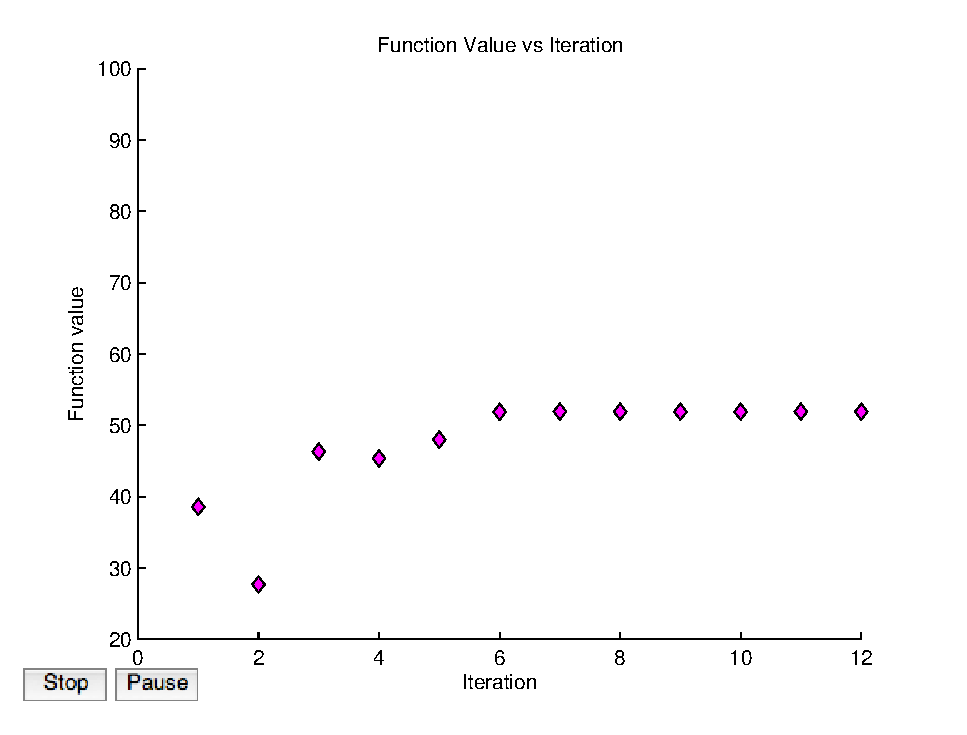
\includegraphics[scale=0.75]{problem1/problem1.eps}
\end{center}

The values of the objective function and design variables at each iteration are shown in Table \ref{Table1}. In addition, the final values of the objective function, design variables, and constraints after convergence of the interior-point algorithm are shown in the Table \ref{Table2}. From these tables, we can see that the optimal value of the function is $51.58233$, which is obtained when $X^T = [-1.049, 0.8736, 2.0485, -0.8113]$.

\begin{table*}[htbp]
	\centering
    \begin{tabular}{|l|l|l|l|l|l|}
        \hline
        Iteration & Function Value & X1 & X2 & X3 & X4\\ \hline
0 & 100 & 0 & 0 & 0 & 0.149\\ 
1 & 31.74371 & -0.118 & 0.0719 & 4.9217 & -1.5518\\ 
2 & 23.33018 & -0.313 & 0.226 & 4.6407 & -2.3259\\ 
3 & 13.32189 & -2.0674 & 2.1062 & 2.765 & -1.1165\\ 
4 & 7.450429 & -2.7524 & 2.1686 & 2.4142 & -0.5794\\ 
5 & 27.82769 & -1.7929 & 1.5429 & 3.1812 & -0.434\\ 
6 & 34.71776 & -1.3829 & 1.0559 & 3.0505 & -0.9692\\ 
7 & 32.77882 & -2.3277 & 0.4378 & 2.0451 & -1.2382\\ 
8 & 49.36069 & -1.5979 & 0.4646 & 1.8595 & -0.9361\\ 
9 & 51.36701 & -1.3108 & 0.6688 & 1.9072 & -0.9095\\ 
10 & 51.06516 & -1.0413 & 0.8928 & 2.0933 & -0.797\\ 
11 & 51.76738 & -1.0257 & 0.8771 & 2.0421 & -0.8189\\ 
12 & 51.58357 & -1.0465 & 0.8699 & 2.0499 & -0.8145\\ 
13 & 51.58272 & -1.0467 & 0.8717 & 2.0495 & -0.8136\\ 
14 & 51.58265 & -1.0494 & 0.8737 & 2.0483 & -0.8112\\ 
15 & 51.58273 & -1.049 & 0.8736 & 2.0484 & -0.8113\\ 
16 & 51.58233 & -1.049 & 0.8736 & 2.0485 & -0.8113\\ 
17 & 51.58233 & -1.049 & 0.8736 & 2.0485 & -0.8113\\ 
        \hline
    \end{tabular}
	\caption{Objective function and design variable values for each iteration during the interior-point algorithm.}
	\label{Table1}
\end{table*}

\begin{table*}[htbp]
	\centering
    \begin{tabular}{|l|l|l|l|l|l|l|l|}
        \hline
	Objective Function & X1 & X2 & X3 & X4 & Constraint 1 & Constraint 2 & Constraint 3 \\ \hline
	51.5823 & -1.049 & 0.8736 & 2.0485 & -0.8113 & -92.3447 & 0 & 0 \\ 
	\hline
    \end{tabular}
	\caption{Final objective function, design variable, and constraint values after convergence of the interior-point algorithm.}
	\label{Table2}
\end{table*}

\begin{problem}{2-a}
\end{problem}
\begin{solution}

Based on the problem description, we seek to optimize the energy stored within the flywheel based on its design specifications, including the maximum permissable mass ($m = 70$ kg), radius ($r = 0.5$ m), rotational speed ($\omega = 3000$ rpm), stress ($\sigma_{max} = 140 x 10^5$ Pa), density ($\rho = 8000$ kg/m$^3$), and Poissons ratio ($v = 0.3$). We are given the equation for the energy of the flywheel as follows:
\begin{eqnarray*}
E & = & \frac{1}{2}I\omega^2 \\
& = & \frac{1}{4}mr^2\omega^2
\end{eqnarray*}
Now, treating the flywheel radius $r$ and width $w$ as design variables, we can re-write $E$ in terms of $r$ and $w$ by making the following observations.
\begin{enumerate}
	\item $E$ is directly proportional to $\omega$, so we will be able to store the maximum energy only when $\omega$ is at its maximum value (that is, $3000$ rpm = $100\pi$ rad/s).
	\item The mass of the flywheel can be derived using the equation for density ($\rho = \frac{m}{v}$), where the volume of the flywheel is equal to that of a cylinder with radius $r$ and height $w$. Thus, after algebraic maniupation, we determine the following:
\begin{eqnarray*}
m = \pi r^2 w \rho
\end{eqnarray*} 
\end{enumerate}
Now, with these two observations, we can treat $\omega$ at its maximal value of $100\pi$ rad/s and substitute $m$ with the expression $m = \pi r^2 w \rho$, since $\rho$ is a fixed value and does not change. Doing this substitution yields the following expression for the energy of the flywheel:
\begin{eqnarray*}
E & = & \frac{1}{4}\pi r^4 w \rho \omega^2 \\
& = & \Big(\frac{8000\pi(100\pi)^2}{4}\Big)r^4 w
\end{eqnarray*}
Now that we have identified the objective that we must optimize, we must establish the constraints on the design variables $r$ and $w$, which are enumerated below:
\begin{enumerate}
	\item From the problem description we are told that $r \leq 0.5$ m.
	\item From the problem description we are told that $m \leq 70$ kg, so replacing $m$ with our previously derived expression $\pi r^2 w \rho$, we know that $\pi r^2 w \rho \leq 70$ kg. Solving this in terms of $r$ and $w$ yields $r^2 w \leq \frac{70}{8000\pi}$ (since $\rho = 8000$ kg/m$^3$).
	\item Based on the distortion energy theory of failure that is used to derive the maximal tangential and radial stresses, and assuming that each of these stresses are equal ($\sigma_t = \sigma_r$), we know that
\begin{eqnarray*}
\sigma_t^2 + \sigma_r^2 - \sigma_t\sigma_r \leq \sigma_{max}^2, 
\end{eqnarray*}
can be reduced to
\begin{eqnarray*}
\frac{1}{2}\rho(3 + v)\omega^2r^2 \leq \sigma_{max}^2.
\end{eqnarray*}
Again, using the fact that $\omega = 100\pi$ rad/s in this maximal case (as well as $v = 0.3$, $\rho = 8000$ kg/m$^3$, and $\sigma_{max} = 140$ x $10^6$ Pa), we can conclude the following:
\begin{eqnarray*}
\frac{8000(3.3)(100\pi)^2}{2}r^2 \leq (140 x 10^6)^2
\end{eqnarray*}
\end{enumerate}
Now, realizing that by maximizing the energy we are minimizing the negation of the energy equation, we can write the problem formally as follows. \\

Minimize
\begin{eqnarray*}
E' = -E = -\Big(\frac{8000\pi(100\pi)^2}{4}\Big)r^4 w
\end{eqnarray*}
subject to the nonlinear constraints:
\begin{enumerate}
	\item $r - 0.5 \leq 0$
	\item $r^2 w  - \frac{70}{8000\pi} \leq 0$
	\item $\frac{8000(3.3)(100\pi)^2}{2}r^2 - (140$ x $10^6)^2 \leq 0$
\end{enumerate}
\end{solution}

\begin{problem}{2-b}
\end{problem}
\begin{solution}
Solving this optimization problem using the $fmincon$ function with the interior-point algorithm yielded the following data for each iteration.

\begin{center}
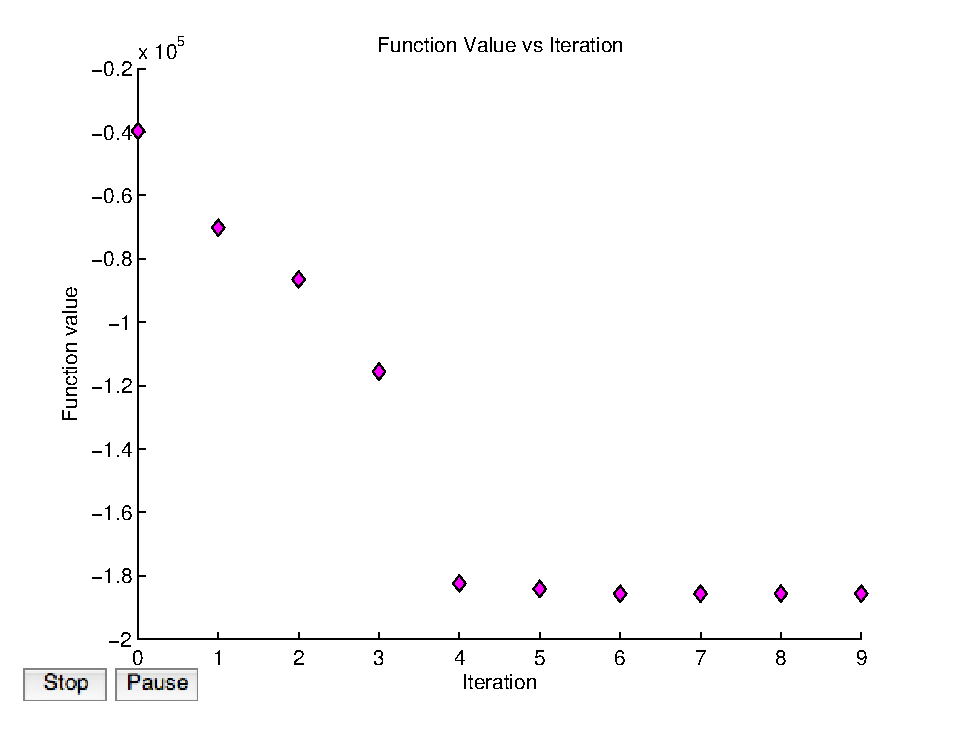
\includegraphics[scale=0.75]{problem2/problem2.eps}
\end{center}

The values of the energy function, radius, and width at each iteration of the interior-point algorithm are shown in Table \ref{Table3}. In addition, the final values of the energy, radius, and width, and constraints after convergence of the interior-point algorithm are shown in the Table \ref{Table4}. It is important to note that since we needed to negate the energy (objective) function to convert it into an appropriate minimization problem for use with the interior-point algorithm, the actual optimal energy value is 185606.1, which is obtained when the radius and width are equal to $0.3278$ m and $0.0259$ m, respectively. 

\begin{table*}[htbp]
	\centering
    \begin{tabular}{|l|l|l|l|}
        \hline
       Iteration & Function Value & Radius & Width\\ \hline
0 & -39688.03 & 0.2 & 0.04\\ 
1 & -70200.94 & 0.2013 & 0.069\\ 
2 & -86527.45 & 0.2395 & 0.0424\\ 
3 & -115583.3 & 0.3154 & 0.0188\\ 
4 & -182378.1 & 0.324 & 0.0267\\ 
5 & -184122.4 & 0.326 & 0.0263\\ 
6 & -185674.5 & 0.3278 & 0.0259\\ 
7 & -185607.6 & 0.3278 & 0.0259\\ 
8 & -185606.1 & 0.3278 & 0.0259\\ 
9 & -185606.1 & 0.3278 & 0.0259\\ 
        \hline
    \end{tabular}
	\caption{Objective function and design variable values for each iteration during the interior-point algorithm.}
	\label{Table3}
\end{table*}

\begin{table*}[htbp]
	\centering
    \begin{tabular}{|l|l|l|l|l|l|}
        \hline
	Objective Function & Radius & Width & Constraint 1 & Constraint 2 & Constraint 3 \\ \hline
	-185606.1 & 0.3278 & 0.0259 & -0.1722 & 0 & -0.0038 \\ 
	\hline
    \end{tabular}
	\caption{Final objective function, design variable, and constraint values after convergence of the interior-point algorithm.}
	\label{Table4}
\end{table*}

\end{solution}

\end{document}
